\documentclass[aspectratio=169]{beamer}

\usetheme{default}
\usecolortheme{default}
\usefonttheme{professionalfonts}

\usepackage[T1]{fontenc}
\usepackage[utf8]{inputenc}
\usepackage{graphicx}
\usepackage{booktabs}
\usepackage{xcolor}
\usepackage{listings}
\usepackage{hyperref}
\usepackage{tikz}
\usetikzlibrary{arrows.meta, positioning, shapes.geometric}

\definecolor{tamumaroon}{HTML}{500000}
\definecolor{tamuwhite}{HTML}{FFFFFF}
\definecolor{tamulight}{HTML}{F7F4F0}
\definecolor{tamugray}{HTML}{3C3C3C}
\definecolor{tamusand}{HTML}{D6D2C4}
\definecolor{cvblue}{HTML}{500000}
\definecolor{cvgreen}{HTML}{3C3C3C}
\definecolor{cvorange}{HTML}{9B6A00}

\lstdefinestyle{slidecode}{
  basicstyle=\ttfamily\tiny,
  breaklines=true,
  breakatwhitespace=false,
  columns=fullflexible,
  keepspaces=true,
  showstringspaces=false,
  frame=single,
  framerule=0.2pt,
  framesep=2pt,
  backgroundcolor=\color{tamuwhite},
  rulecolor=\color{tamusand},
  aboveskip=0.05cm,
  belowskip=0.05cm,
  xleftmargin=0pt,
  xrightmargin=0pt
}

\setbeamercolor{normal text}{fg=tamugray,bg=tamuwhite}
\setbeamercolor{title}{fg=tamumaroon}
\setbeamercolor{frametitle}{fg=tamuwhite,bg=tamumaroon}
\setbeamercolor{structure}{fg=tamumaroon}
\setbeamercolor{block title}{fg=tamuwhite,bg=tamumaroon}
\setbeamercolor{block body}{fg=tamugray,bg=tamulight}
\setbeamercolor{author in head/foot}{fg=tamuwhite,bg=tamumaroon}
\setbeamercolor{title in head/foot}{fg=tamuwhite,bg=tamumaroon}
\setbeamercolor{date in head/foot}{fg=tamuwhite,bg=tamumaroon}
\setbeamercolor{item}{fg=tamumaroon}
\setbeamercolor{subitem}{fg=tamumaroon}
\setbeamerfont{title}{size=\Large}
\setbeamerfont{author}{size=\small}
\setbeamerfont{date}{size=\footnotesize}
\setbeamerfont{frametitle}{size=\large,series=\bfseries}
\setbeamerfont{block title}{size=\small,series=\bfseries}
\setbeamerfont{block body}{size=\small}
\setbeamertemplate{navigation symbols}{}
\setbeamertemplate{itemize item}{\color{tamumaroon}\small$\blacktriangleright$}
\setbeamertemplate{itemize subitem}{\color{tamumaroon}\scriptsize$\bullet$}
\setbeamertemplate{blocks}[rounded][shadow=false]
\setbeamertemplate{frametitle}{
  \vspace{0.25cm}
  {\color{tamumaroon}\insertframetitle}
  \par\vspace{0.1cm}
  {\color{tamumaroon}\rule{\textwidth}{0.6pt}}
}
\setbeamertemplate{footline}{
  \leavevmode
  \hbox{
    \begin{beamercolorbox}[wd=.68\paperwidth,ht=2.5ex,dp=1ex,leftskip=0.25cm]{author in head/foot}
      Henry Ruiz, PhD \hspace{0.2cm} | \hspace{0.2cm} Texas A\&M University
    \end{beamercolorbox}
    \begin{beamercolorbox}[wd=.27\paperwidth,ht=2.5ex,dp=1ex,rightskip=0.25cm plus1fil]{date in head/foot}
      \hfill \insertframenumber/\inserttotalframenumber
    \end{beamercolorbox}
  }
}

\title[VisionOps Crew]{Building VisionOps Crew\\Using Google ADK, MCP, Jupyter, and Antigravity}
\subtitle{}
\author[Henry Ruiz, PhD]{\texorpdfstring{Henry Ruiz, PhD\\Research Scientist, Texas A\&M University\\GDE in AI \& Cloud\\@devharuiz\\\href{https://haruiz.github.io/}{haruiz.github.io}}{Henry Ruiz, PhD, Research Scientist, Texas A and M University, GDE in AI and Cloud, @devharuiz, haruiz.github.io}}
\date{\today}
\hypersetup{
  pdftitle={Building VisionOps Crew Using Google ADK, MCP, Jupyter, and Antigravity},
  pdfauthor={Henry Ruiz, PhD},
  pdfsubject={Developer workshop on multi-agent computer vision systems},
  pdfkeywords={computer vision, Google ADK, Hugging Face, Voxel51, Jupyter MCP, Antigravity SDK, MCP, agents}
}

\begin{document}

\begin{frame}[plain]
  \vspace{0.25cm}
  {\color{tamumaroon}\rule{\textwidth}{1.2pt}}\\[0.45cm]
  {\LARGE\color{tamumaroon}\textbf{Building VisionOps Crew}}\\[0.18cm]
  {\large\color{tamugray}Using Google ADK, MCP, Jupyter, and Antigravity}\\[0.45cm]
  {\small
  \textbf{Henry Ruiz, PhD}\\
  Research Scientist, Texas A\&M University\\
  GDE in AI \& Cloud\\
  @devharuiz \quad \href{https://haruiz.github.io/}{haruiz.github.io}
  }

  \vfill
  \begin{block}{Workshop goal}
    \small
    Learn how to build a Google ADK multi-agent system that can reason through a computer vision task, discover relevant models and datasets from Hugging Face, inspect data with FiftyOne/Voxel51, prototype with Jupyter MCP, and use Antigravity SDK as an opt-in implementation and artifact-generation tool.
  \end{block}
  {\color{tamumaroon}\rule{\textwidth}{0.6pt}}
\end{frame}

\begin{frame}{Background: What Is Computer Vision?}
  \begin{block}{Definition}
    \small
    Computer vision is the field of building systems that extract structured
    information from images, video, and visual sensor streams.
  \end{block}
  \vspace{0.3cm}
  \small
  Visual data is usually converted into:
  \begin{itemize}
    \item labels, detections, masks, keypoints, embeddings, or captions
    \item model outputs that can be evaluated, debugged, and deployed
    \item workflows that connect data, models, metrics, and applications
  \end{itemize}
\end{frame}

\begin{frame}{Common Computer Vision Tasks}
  \centering
  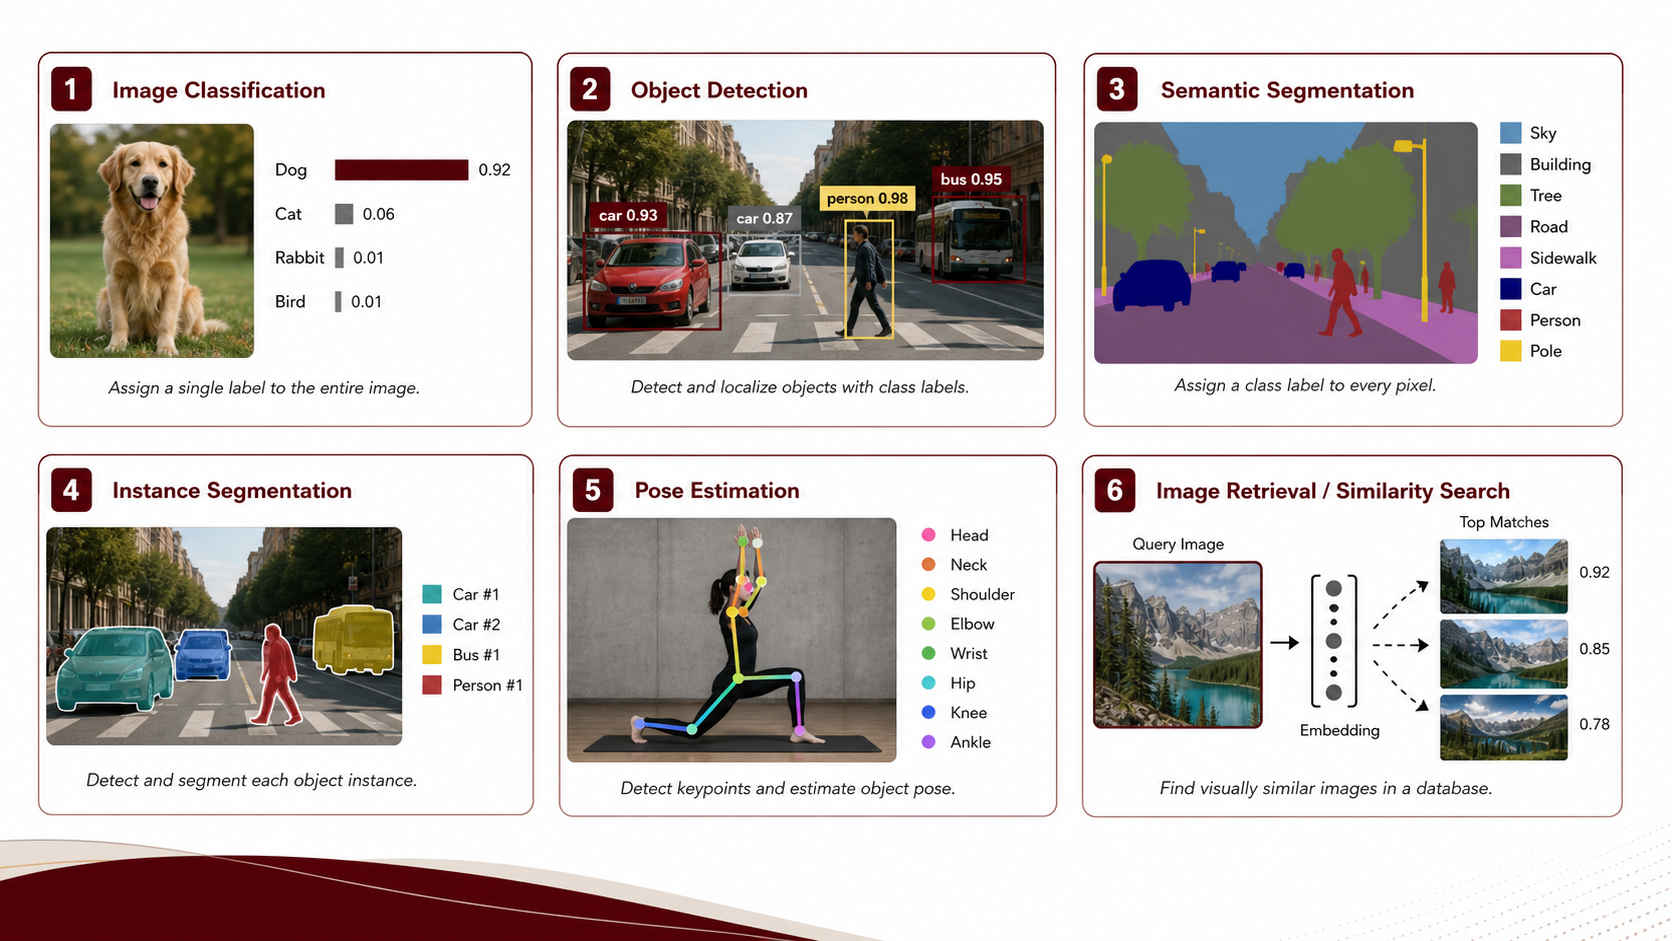
\includegraphics[height=0.66\textheight]{../../assets/common_cv_tasks.png}

  \vspace{0.02cm}
  {\tiny\color{tamugray}The expert agent should recognize task type early:
  task classification drives dataset inspection, model search, metrics, and
  implementation choices.}
\end{frame}

\begin{frame}{Background: Traditional CV Pipeline}
  \centering
  \small
  \resizebox{0.96\textwidth}{!}{%
  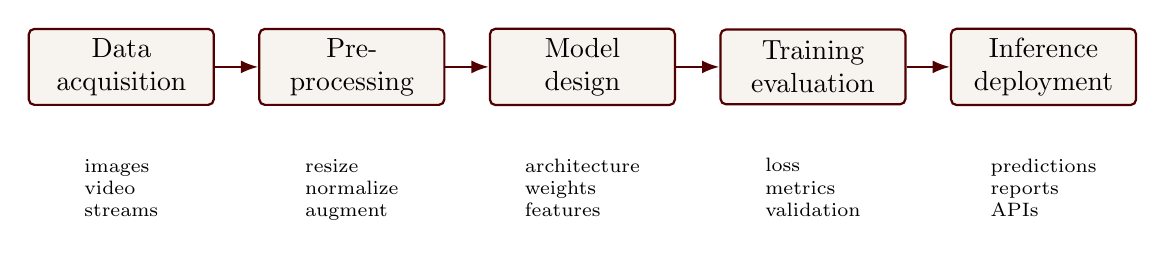
\begin{tikzpicture}[
    stage/.style={
      rectangle,
      rounded corners=2pt,
      draw=tamumaroon,
      thick,
      align=center,
      minimum width=2.35cm,
      minimum height=0.95cm,
      fill=tamulight
    },
    arrow/.style={-{Latex[length=2.2mm]}, thick, draw=tamumaroon}
  ]
    \node[stage] (data) {Data\\acquisition};
    \node[stage, right=0.55cm of data] (prep) {Pre-\\processing};
    \node[stage, right=0.55cm of prep] (model) {Model\\design};
    \node[stage, right=0.55cm of model] (train) {Training\\evaluation};
    \node[stage, right=0.55cm of train] (infer) {Inference\\deployment};

    \draw[arrow] (data) -- (prep);
    \draw[arrow] (prep) -- (model);
    \draw[arrow] (model) -- (train);
    \draw[arrow] (train) -- (infer);

    \node[below=0.55cm of data, align=left, font=\scriptsize] {images\\video\\streams};
    \node[below=0.55cm of prep, align=left, font=\scriptsize] {resize\\normalize\\augment};
    \node[below=0.55cm of model, align=left, font=\scriptsize] {architecture\\weights\\features};
    \node[below=0.55cm of train, align=left, font=\scriptsize] {loss\\metrics\\validation};
    \node[below=0.55cm of infer, align=left, font=\scriptsize] {predictions\\reports\\APIs};
  \end{tikzpicture}%
  }

  \vspace{0.65cm}
  \begin{block}{Key idea}
    \small
    Each stage depends on the previous one. Many errors come from mismatches
    between the data, labels, preprocessing, model choice, and evaluation
    metric.
  \end{block}
\end{frame}

\begin{frame}{Tools For Computer Vision Workflows}
  \begin{columns}[T,onlytextwidth]
    \begin{column}{0.48\textwidth}
      \small
      \begin{block}{Core development}
        \scriptsize
        \begin{itemize}
          \item \textbf{OpenCV}: classic image and video processing toolkit for
          filtering, transforms, feature extraction, camera I/O, and quick
          preprocessing prototypes.
          \item \textbf{PyTorch + torchvision}: deep learning stack for model
          training, transfer learning, datasets, transforms, and reusable
          vision model components.
          \item \textbf{Ultralytics YOLO}: production-friendly object detection,
          segmentation, and tracking workflows with pretrained models and
          simple training/export commands.
        \end{itemize}
      \end{block}
    \end{column}
    \begin{column}{0.48\textwidth}
      \small
      \begin{block}{Model and data discovery}
        \scriptsize
        \begin{itemize}
          \item \textbf{Hugging Face}: hub for pretrained models, datasets,
          demos, papers, and documentation across classification, detection,
          segmentation, captioning, and multimodal tasks.
          \item \textbf{FiftyOne / Voxel51}: dataset inspection platform for
          visualizing samples, labels, embeddings, mistakes, slices, and model
          predictions before committing to training decisions.
        \end{itemize}
      \end{block}
      \vspace{0.12cm}
      {\scriptsize\color{tamugray}Agents can coordinate these tools: inspect
      data locally, search for models, choose baselines, and turn findings into
      concrete engineering next steps.}
    \end{column}
  \end{columns}
\end{frame}

\begin{frame}{Why Automate The Pipeline With Agents?}
  \begin{columns}[T,onlytextwidth]
    \begin{column}{0.48\textwidth}
      \small
      \textbf{Automation advantages}
      \vspace{0.15cm}
      \begin{itemize}
        \item Route ambiguous requests to the right specialist tools
        \item Combine external model research with local dataset evidence
        \item Preserve context across pipeline stages and specialized tasks
        \item Make tool calls observable, traceable, and reproducible
        \item Generate actionable next steps for implementation and deployment
      \end{itemize}
    \end{column}
    \begin{column}{0.48\textwidth}
      \begin{block}{Important distinction}
        \small
        Agents do not replace human judgment. They help coordinate repeated
        steps: planning, research, dataset inspection, and workflow synthesis.
      \end{block}
    \end{column}
  \end{columns}
\end{frame}

\begin{frame}{Project Intro: VisionOps Crew}
  \centering
  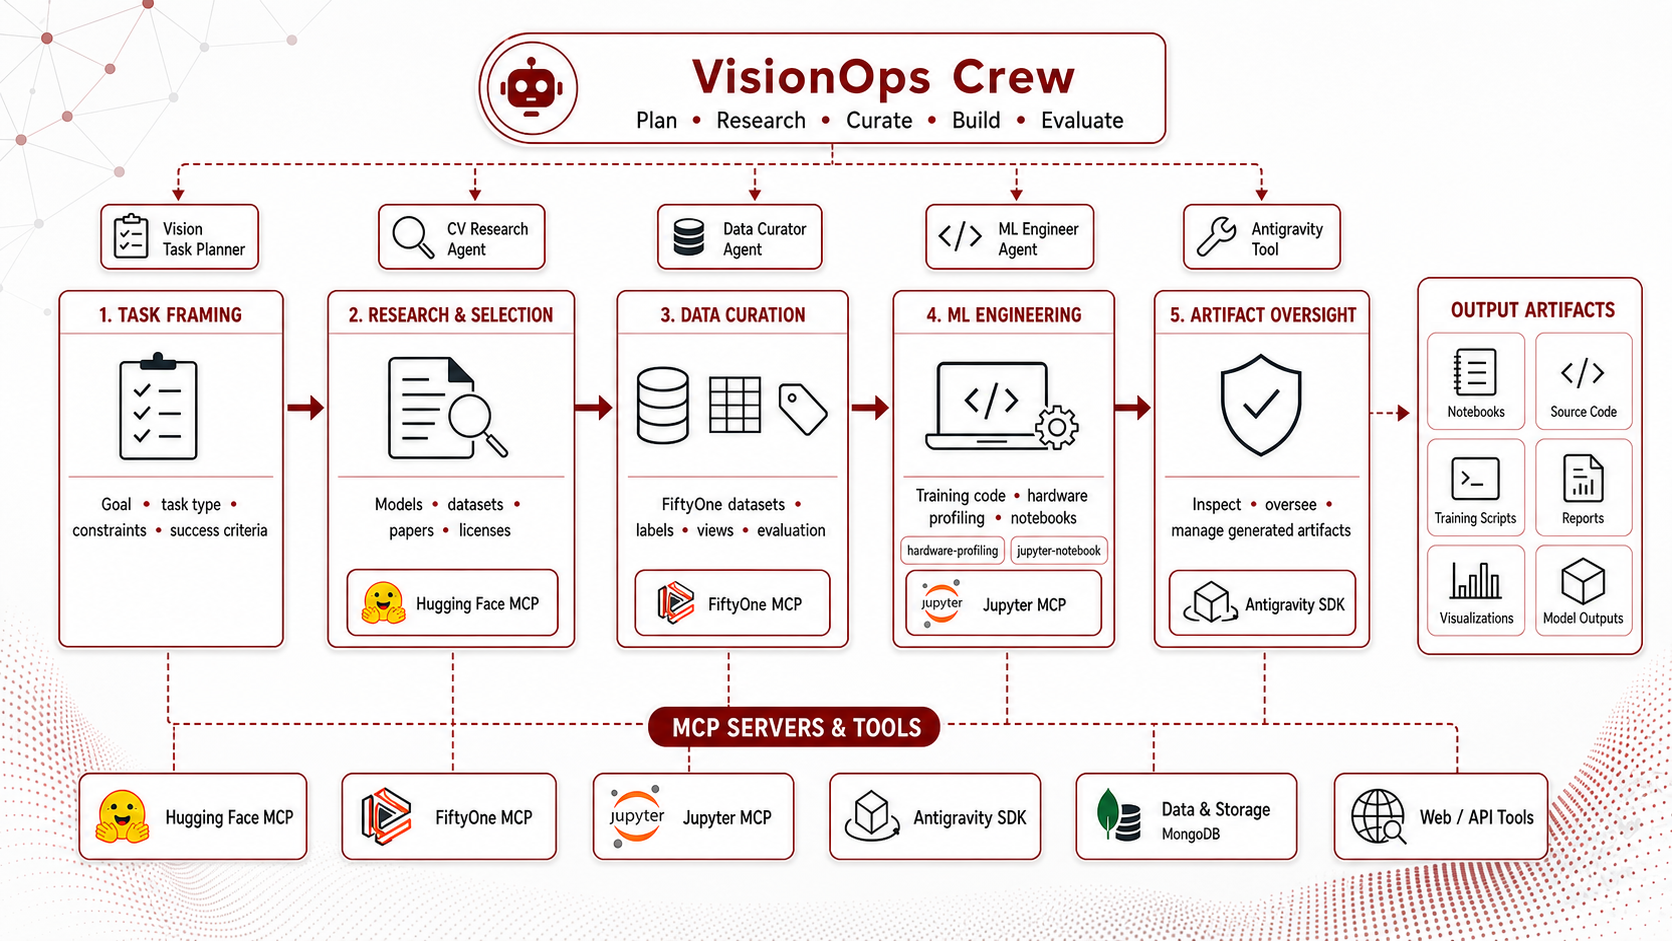
\includegraphics[height=0.76\textheight]{../../assets/visionops_workflow_artifacts.png}
\end{frame}

\begin{frame}{Multi-Agent Architecture: Agents}
  \small
  \textbf{System design pattern:} one ADK orchestrator, specialist agents,
  and clear tool boundaries.
  \vspace{0.15cm}
  \begin{itemize}
    \item \textbf{Google ADK orchestrator}: routes the request and combines
    the specialists' results.
    \item \textbf{Vision planner}: identifies the task type, assumptions,
    constraints, risks, and success criteria.
    \item \textbf{CV research agent}: searches models, datasets, Spaces, papers,
    documentation, and licenses.
    \item \textbf{Data curator agent}: works with local FiftyOne datasets,
    schemas, labels, filters, views, and App state.
    \item \textbf{ML engineer agent}: turns outputs into training, evaluation,
    debugging, hardware-aware implementation steps, and Jupyter notebook
    prototypes.
    \item \textbf{Antigravity tool}: opt-in direct orchestrator tool for code,
    images, reports, notebooks, and generated artifacts.
  \end{itemize}
\end{frame}

\begin{frame}{Multi-Agent Architecture: Diagram}
  \centering
  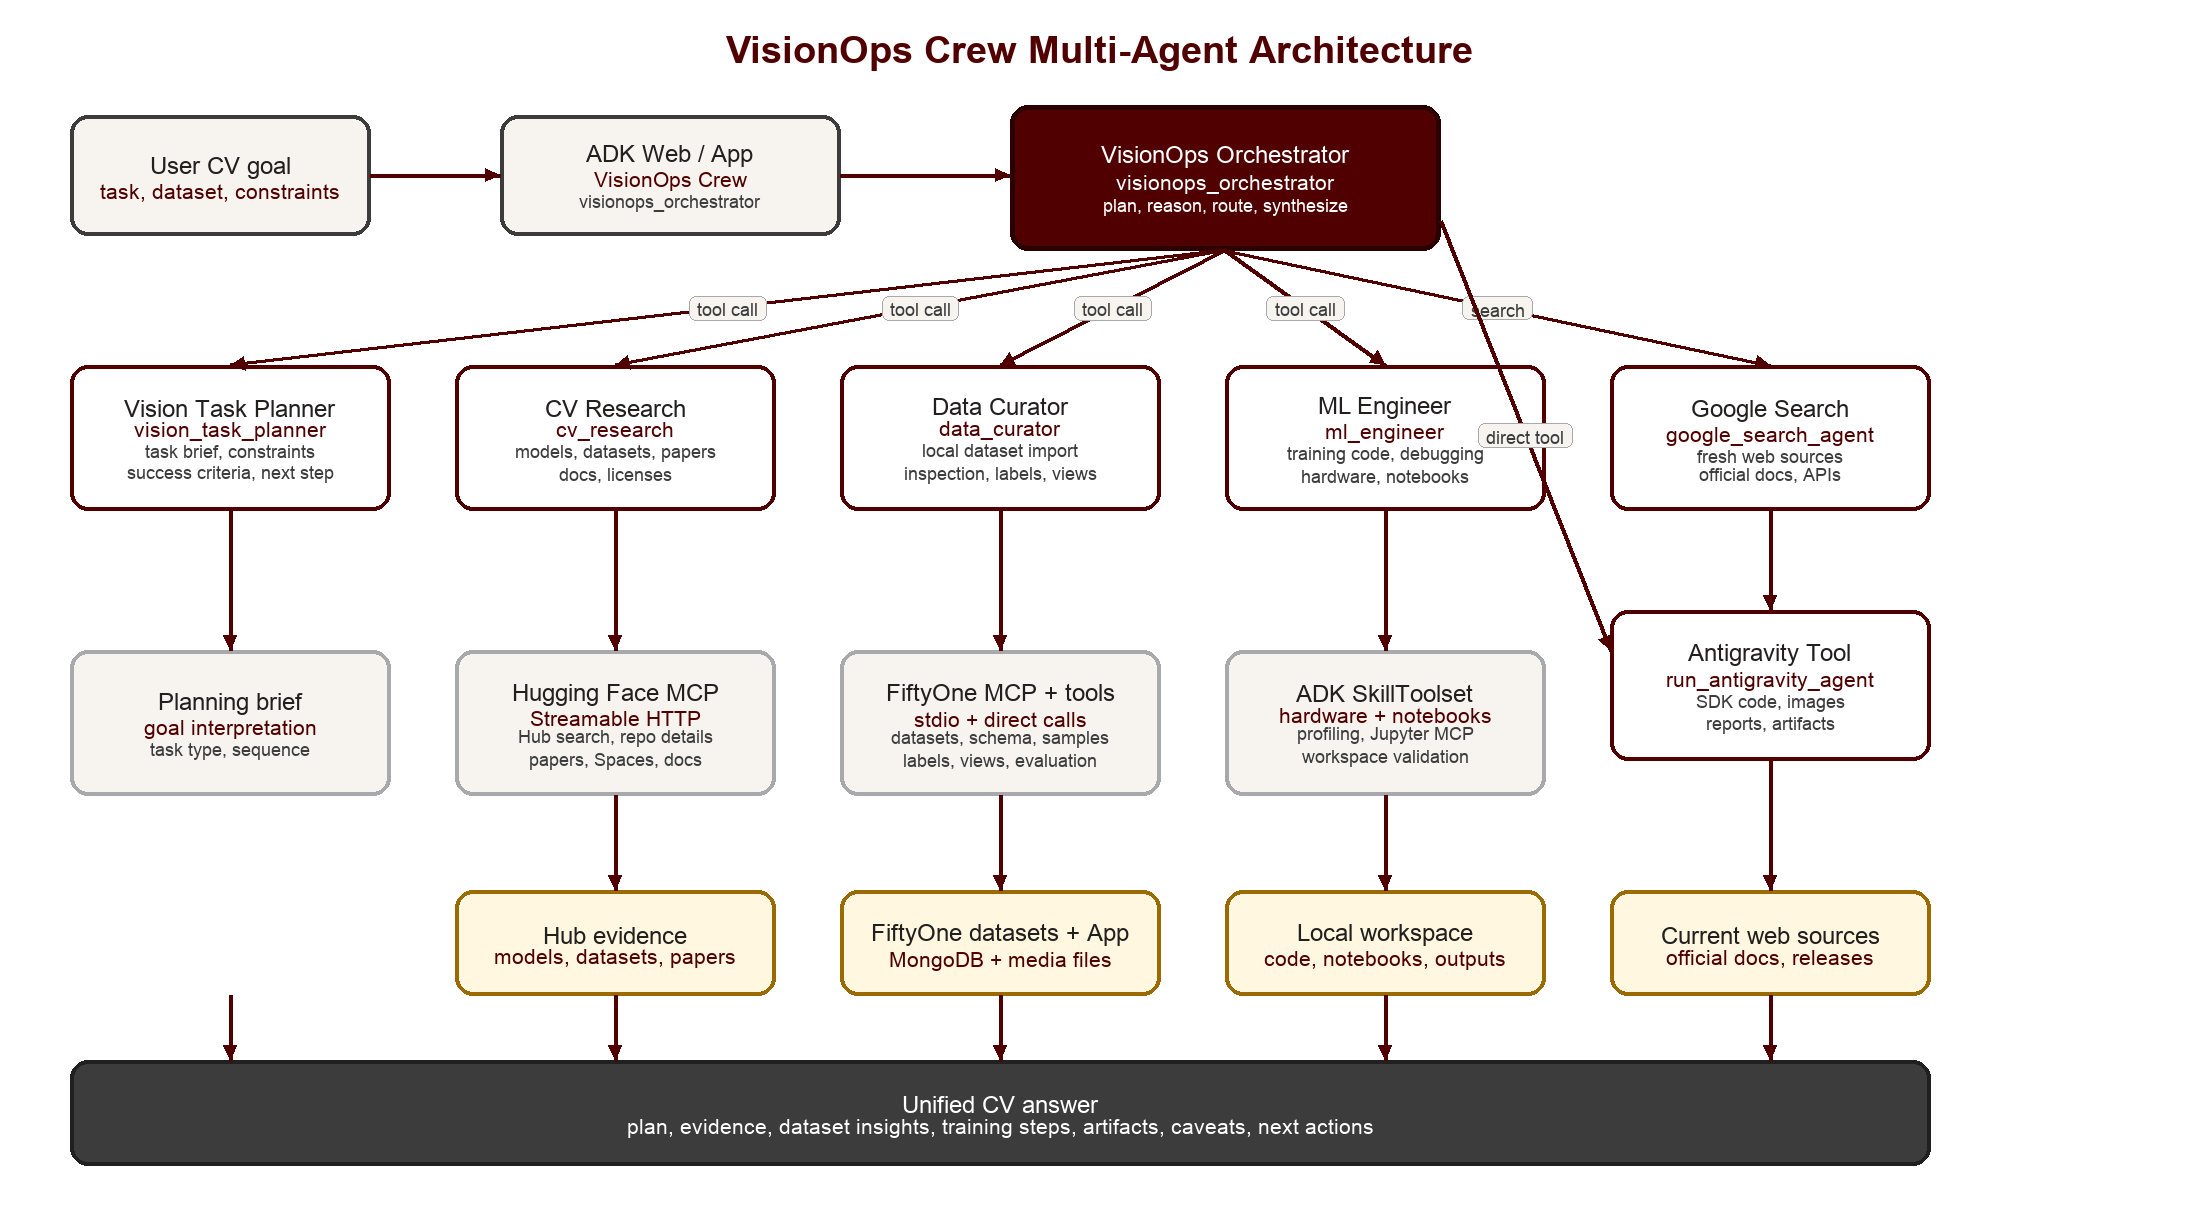
\includegraphics[height=0.67\textheight]{../../assets/visionops_multi_agent_architecture.png}

  \vspace{0.05cm}
  {\scriptsize\color{tamugray}Google ADK coordinates the agents. MCP servers
  connect the system to Hugging Face, FiftyOne, Jupyter, and local tools. Antigravity
  is a direct opt-in orchestrator tool, not an ML Engineer skill.}
\end{frame}

\begin{frame}[fragile]{Jupyter MCP In The ML Engineer}
  \begin{columns}[T,onlytextwidth]
    \begin{column}{0.48\textwidth}
      \small
      \textbf{Why notebooks matter}
      \vspace{0.12cm}
      \begin{itemize}
        \item Keep exploratory ML work in durable \texttt{.ipynb} artifacts
        \item Create, open, edit, execute, and inspect notebook cells through MCP
        \item Store plots, metrics, data checks, and training notes next to code
        \item Separate notebook work from one-off shell snippets
      \end{itemize}
    \end{column}
    \begin{column}{0.48\textwidth}
      \begin{block}{ADK wiring}
\begin{lstlisting}[style=slidecode]
jupyter_mcp_toolset = McpToolset(
    connection_params=StdioConnectionParams(
        server_params=StdioServerParameters(
            command="uvx",
            args=["jupyter-mcp-server@latest"],
            env=jupyter_mcp_env,
        ),
        timeout=30.0,
    )
)
\end{lstlisting}
      \end{block}
      \vspace{0.05cm}
      {\scriptsize\color{tamugray}The \texttt{jupyter-notebook} skill instructs
      the ML Engineer to prefer notebook MCP tools for exploratory coding,
      visualization, and scientific computing.}
    \end{column}
  \end{columns}
\end{frame}

\begin{frame}[fragile]{Antigravity SDK As An Opt-In Orchestrator Tool}
  \begin{columns}[T,onlytextwidth]
    \begin{column}{0.48\textwidth}
      \small
      \textbf{Placement in the system}
      \vspace{0.12cm}
      \begin{itemize}
        \item Exposed as \texttt{run\_antigravity\_agent} on the root orchestrator
        \item Used only when the user explicitly asks for Antigravity
        \item Can generate images, code suggestions, notebooks, reports, and scaffolds
        \item Tracks concrete created/updated artifacts from configured roots
        \item Denies file writes unless the user confirms the exact write action
      \end{itemize}
    \end{column}
    \begin{column}{0.48\textwidth}
      \begin{block}{SDK pattern}
\begin{lstlisting}[style=slidecode]
config = LocalAgentConfig(
    system_instructions=(
        ANTIGRAVITY_EXPERT_INSTRUCTIONS
    ),
    model=os.getenv("ANTIGRAVITY_MODEL",
                    "gemini-3.5-flash"),
    workspaces=[str(REPO_ROOT)],
    api_key=os.getenv("GEMINI_API_KEY"),
    save_dir=str(
        ANTIGRAVITY_SESSIONS_DIR / "expert"
    ),
    app_data_dir=str(ANTIGRAVITY_APP_DATA_DIR),
)

async with Agent(config) as agent:
    response = await agent.chat(task)
    result = await response.text()
\end{lstlisting}
      \end{block}
    \end{column}
  \end{columns}
\end{frame}

\begin{frame}{Test Example: From Prompt To Output}
  \centering
  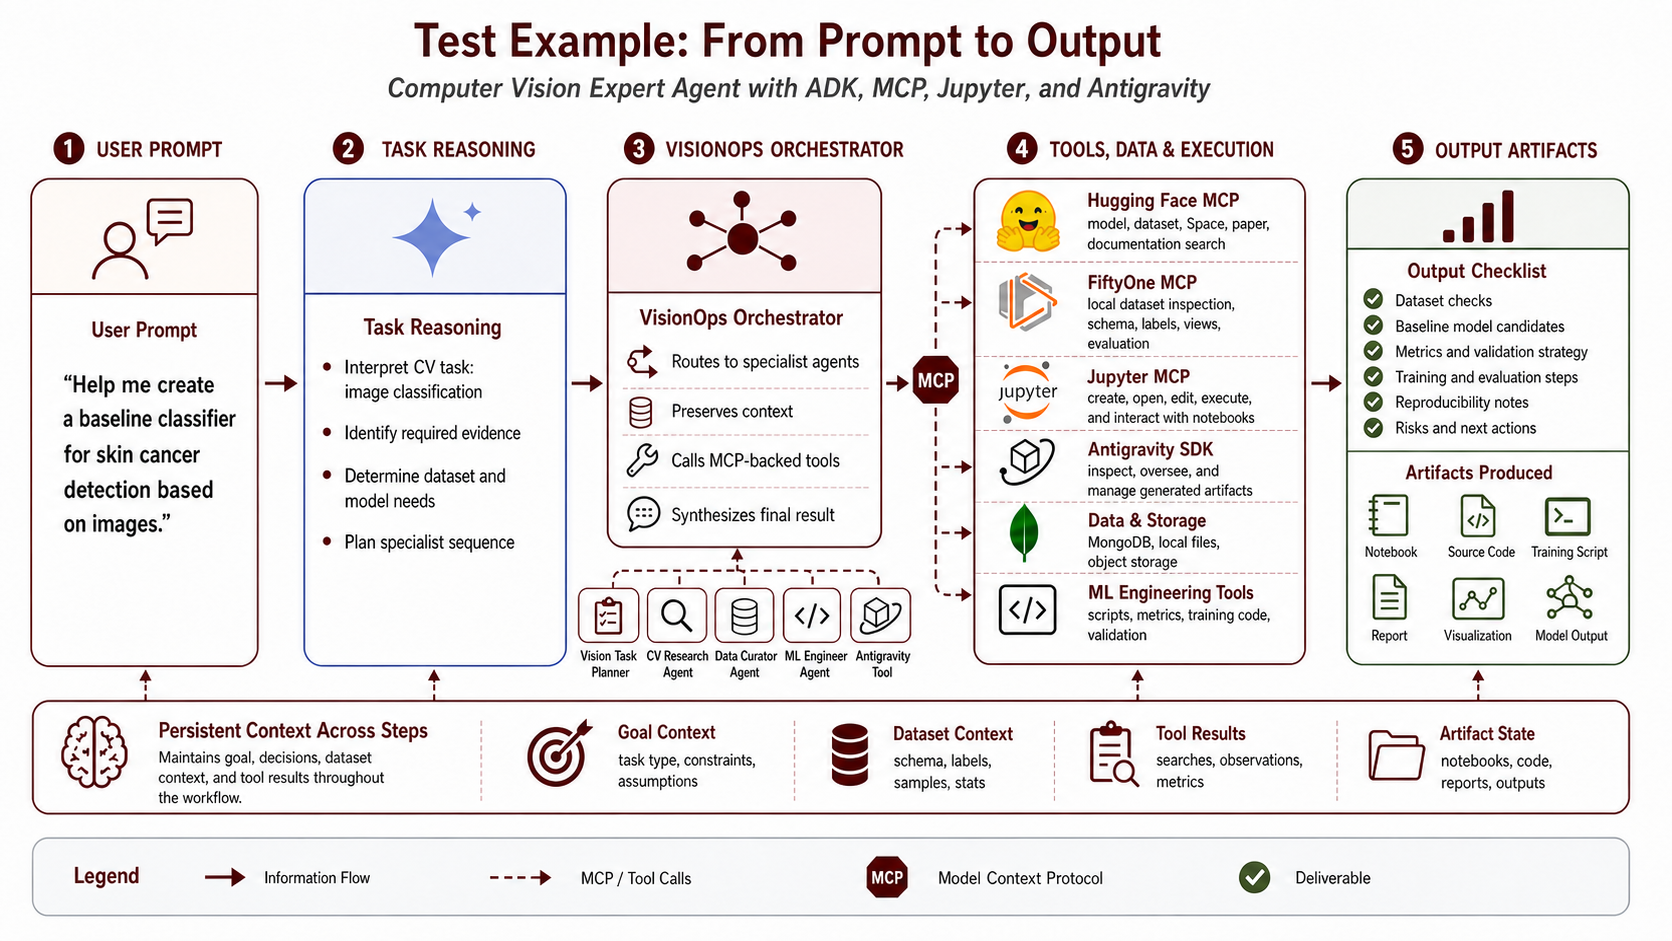
\includegraphics[height=0.76\textheight]{../../assets/test_example_prompt_to_output.png}
\end{frame}

\begin{frame}[plain]
  \centering
  \vspace{0.6cm}
  {\color{tamumaroon}\rule{0.75\textwidth}{1.2pt}}\\[0.65cm]
  {\Huge\color{tamumaroon}\textbf{Thank You}}\\[0.45cm]
  {\Large Questions and Discussion}\\[0.75cm]

  {\large\textbf{Henry Ruiz, PhD}}\\[0.15cm]
  Research Scientist, Texas A\&M University\\
  GDE in AI \& Cloud\\[0.35cm]
  @devharuiz\\
  \href{https://haruiz.github.io/}{haruiz.github.io}\\[0.65cm]
  {\color{tamumaroon}\rule{0.75\textwidth}{0.6pt}}
\end{frame}

\end{document}
